\chapter{Introducción Específica} % Main chapter title
%----------------------------------------------------------------------------------------
%	SECTION 1
%----------------------------------------------------------------------------------------
A fin de comprender las decisiones que se adoptaron al momento de definir la arquitectura del software, es necesario comprender el entorno del problema, los casos de uso y requerimientos del sistema. 

\section{Problemática}
\subsection{Entorno del sistema}

En la linea de galvanizado original los técnicos operaban en un ambiente altamente corrosivo por los vapores emanados de las soluciones, y con en el soporte de instrumental de medición muy básico para utilizar en algunos de las etapas en la linea.
En las diferentes bateas de la linea de galvanizado se necesitaban controlar distintos combinación de los siguientes parámetros:
\begin{itemize}
	\item Temperatura.
	\item Nivel de líquidos.
	\item Conductividad o concentración de iones.
	\item Corriente entregada (electrolisis).
	\item Inyección de aire.
\end{itemize}

Debido a que la linea cuenta con varias bateas distintas colocadas en forma consecutiva se planteo la necesidad de en primer lugar de que el sistema debía ser capaz de manejar, en función de parámetros específicos a cada etapa, el conjunto de estos parámetros como un solo núcleo de procesamiento con los sensores y actuadores colocados en una sola cuba de prueba. A su vez era necesario contar con la capacidad de manejar diversas señales de interruptores y actuadores de interacción con el operario.
En función del éxito de este banco la expansión a futuro con módulos de entrada y salida a lo largo de la planta, se implementaría en otra etapa.

\subsection{Casos de Uso}

Como primera instancia fue necesario conocer los casos de uso a los cuales vincularan al usuario y al sistema en función de la operación a ejecutar. Para ello se definieron tres casos globales:
\begin{enumerate}
	\item Puesta en alta del dispositivo.
	\item Operación en modo de funcionamiento 1.
	\item Operación en modo de funcionamiento 2.
\end{enumerate}

En la Figuras \ref{fig:casoUsoAlta} y \ref{fig:casodeUso1y2} se notan las interacciones entre los distintos submódulos del sistema en función de los casos de usos determinados por los operadores.

\begin{figure}[h!]
	\centering
	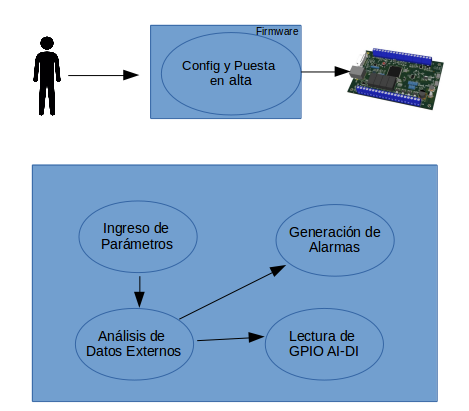
\includegraphics[width=.8\textwidth]{Figures/caso_uso_1y2_UML}
	\caption{Diagrama UML de casos de uso Modo 1 y 2.}
	\label{fig:casodeUso1y2}
\end{figure}

\begin{figure}[h!]
	\centering
	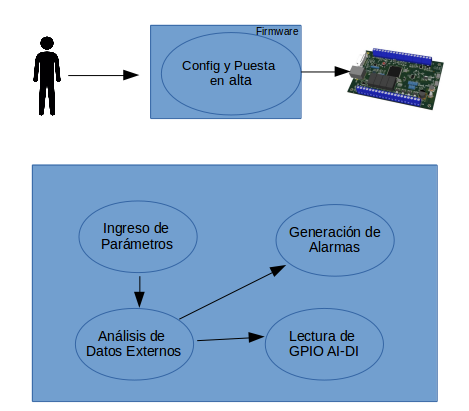
\includegraphics[width=.8\textwidth]{Figures/caso_uso_Alta_UML}
	\caption{Diagrama UML caso de uso de puesta en alta.}
	\label{fig:casoUsoAlta}
\end{figure}


\section{Requerimientos}
\label{sec:Requerimientos}

% Ver si conviene listar todos los requerimientos otra vez o solo los mas determinates.

Se recomienda no utilizar \textbf{texto en negritas} en ningún párrafo, ni tampoco texto \underline{subrayado}. En cambio sí se sugiere utilizar \textit{texto en cursiva} donde se considere apropiado.

Se sugiere que la escritura sea impersonal. Por ejemplo, no utilizar ``el diseño del firmware lo hice de acuerdo con tal principio'', sino ``el firmware fue diseñado utilizando tal principio''. En lo posible hablar en tiempo pasado, ya que la memoria describe un trabajo que ya fue realizado.

Se recomienda no utilizar una sección de glosario sino colocar la descripción de las abreviaturas como parte del mismo cuerpo del texto. Por ejemplo, RTOS (\textit{Real Time Operating System}, Sistema Operativo de Tiempo Real) o en caso de considerarlo apropiado mediante notas a pie de página.

Si se desea indicar alguna página web utilizar el siguiente formato de referencias bibliográficas, dónde las referencias se detallan en la sección de bibliografía de la memoria,utilizado el formato establecido por IEEE en \citep{IEEE:citation}. Por ejemplo, ``el presente trabajo se basa en la plataforma EDU-CIAA-NXP, la cual se describe en detalle en \citep{CIAA}''.

\section{Planificación} 

Con propósito de cumplir con las metas de tiempo planteadas, se realizo una planificación de tareas según los hitos mas importantes y la interrelación según la dependencia de ejecución. En la Figura \ref{fig:WBStareas} se resumen el diagrama de tareas del proyecto.
Además del diagrama se desarrollo una planificacion temporal la cual se observa en el diagrama de Gantt (Colocar referencia) que se nota en la Figura \ref{fig:Ganttareas}.

\begin{figure}[h!]
	\centering
	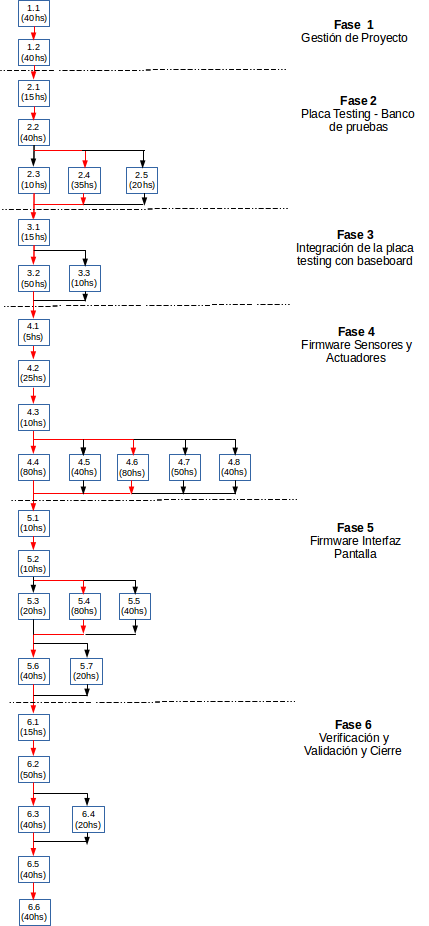
\includegraphics[scale=.8]{Figures/WBS_tareas}
	\caption{Diagrama de tareas del proyecto completo.\protect\footnotemark.}
	\label{fig:WBStareas}
\end{figure}

\begin{figure}[h!]
	\centering
	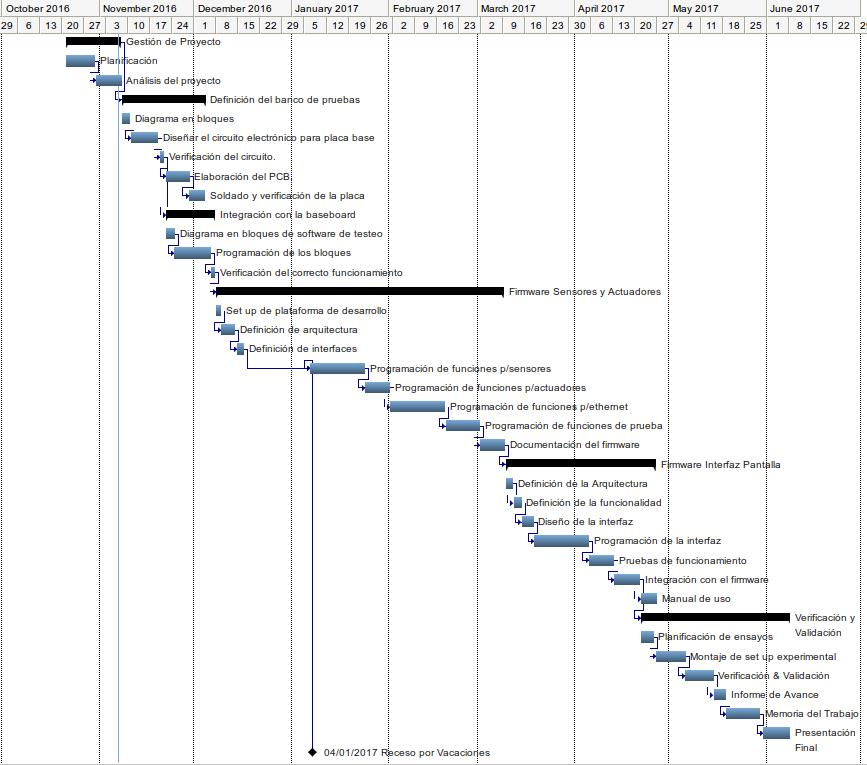
\includegraphics[scale=.5]{Figures/Gantt_tareas}
	\caption{Diagrama de Gantt del proyecto completo.\protect\footnotemark.}
	\label{fig:Ganttareas}
\end{figure}

El texto de las figuras debe estar siempre en español, excepto que se decida reproducir una figura original tomada de alguna referencia. En ese caso la referencia de la cual se tomó la figura debe ser indicada en el epígrafe de la figura e incluida como una nota al pie, como se ilustra en la figura \ref{fig:palabraIngles}.
\footnotetext{\url{https://goo.gl/images/i7C70w}}


\subsection{Tablas}

Para las tablas utilizar el mismo formato que para las figuras, sólo que el epígrafe se debe colocar arriba de la tabla, como se ilustra en la tabla \ref{tab:peces}. Observar que sólo algunas filas van con líneas visibles y notar el uso de las negritas para los encabezados.  La referencia se logra utilizando el comando \verb|\ref{<label>}| donde label debe estar definida dentro del entorno de la tabla.

\begin{table}[h]
	\centering
	\caption[caption corto]{caption largo más descriptivo}
	\begin{tabular}{l c c}    
		\toprule
		\textbf{Especie} 	 & \textbf{Tamaño}  & \textbf{Valor aprox.}  \\
		\midrule
		Amphiprion Ocellaris	 & 10 cm 			& \$ 6.000 \\		
		Hepatus Blue Tang	 & 15 cm				& \$ 7.000 \\
		Zebrasoma Xanthurus	 & 12 cm				& \$ 6.800 \\
		\bottomrule
		\hline
	\end{tabular}
	\label{tab:peces}
\end{table}


\subsection{Ecuaciones}
\label{sec:Ecuaciones}

Al insertar ecuaciones en la memoria estas se deben numerar de la siguiente forma:

\begin{equation}
	\label{eq:metric}
	ds^2 = c^2 dt^2 \left( \frac{d\sigma^2}{1-k\sigma^2} + \sigma^2\left[ d\theta^2 + \sin^2\theta d\phi^2 \right] \right)
\end{equation}
                                                        
Es importante tener presente que en el caso de las ecuaciones estas pueden ser referidas por su número, como por ejemplo ``tal como describe la ecuación \ref{eq:metric}'', pero también es correcto utilizar los dos puntos, como por ejemplo ``la expresión matemática que describe este comportamiento es la siguiente:''

\begin{equation}
	\label{eq:schrodinger}
	\frac{\hbar^2}{2m}\nabla^2\Psi + V(\mathbf{r})\Psi = -i\hbar \frac{\partial\Psi}{\partial t}
\end{equation}

Para las ecuaciones se debe utilizar un tamaño de letra equivalente al utilizado para el texto del trabajo, en tipografía cursiva y preferentemente del tipo Times New Roman o similar. El espaciado antes y después de cada ecuación es de aproximadamente el doble que entre párrafos consecutivos del cuerpo principal del texto. Por suerte la plantilla se encarga de esto por nosotros.

Y para la ecuación \ref{eq:schrodinger}:

\begin{verbatim}
\begin{equation}
	\label{eq:schrodinger}
	\frac{\hbar^2}{2m}\nabla^2\Psi + V(\mathbf{r})\Psi = 
	-i\hbar \frac{\partial\Psi}{\partial t}
\end{equation}

\end{verbatim}